% Created by tikzDevice version 0.12 on 2019-03-07 11:08:25
% !TEX encoding = UTF-8 Unicode
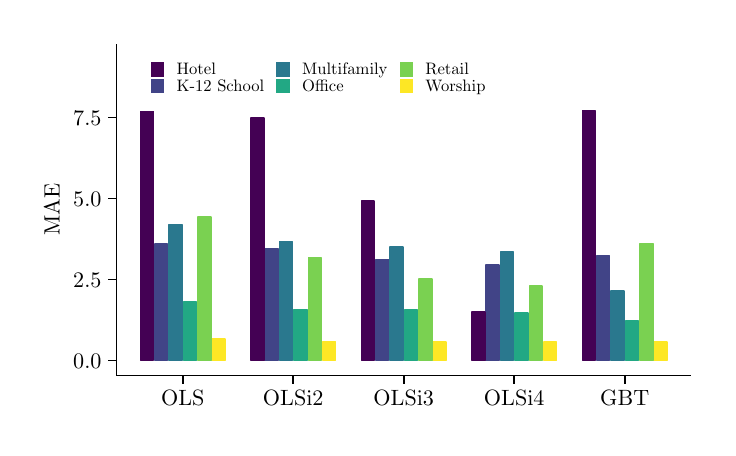
\begin{tikzpicture}[x=1pt,y=1pt]
\definecolor{fillColor}{RGB}{255,255,255}
\path[use as bounding box,fill=fillColor,fill opacity=0.00] (0,0) rectangle (245.72,144.54);
\begin{scope}
\path[clip] (  0.00,  0.00) rectangle (245.72,144.54);
\definecolor{drawColor}{RGB}{255,255,255}
\definecolor{fillColor}{RGB}{255,255,255}

\path[draw=drawColor,line width= 0.6pt,line join=round,line cap=round,fill=fillColor] (  0.00,  0.00) rectangle (245.72,144.54);
\end{scope}
\begin{scope}
\path[clip] ( 32.07, 18.85) rectangle (239.72,138.54);
\definecolor{fillColor}{RGB}{255,255,255}

\path[fill=fillColor] ( 32.07, 18.85) rectangle (239.72,138.54);
\definecolor{drawColor}{RGB}{253,231,37}
\definecolor{fillColor}{RGB}{253,231,37}

\path[draw=drawColor,line width= 0.6pt,line join=round,fill=fillColor] ( 66.68, 24.29) rectangle ( 71.34, 32.02);
\definecolor{drawColor}{RGB}{122,209,81}
\definecolor{fillColor}{RGB}{122,209,81}

\path[draw=drawColor,line width= 0.6pt,line join=round,fill=fillColor] ( 61.49, 24.29) rectangle ( 66.15, 76.01);
\definecolor{drawColor}{RGB}{34,168,132}
\definecolor{fillColor}{RGB}{34,168,132}

\path[draw=drawColor,line width= 0.6pt,line join=round,fill=fillColor] ( 56.30, 24.29) rectangle ( 60.96, 45.35);
\definecolor{drawColor}{RGB}{42,120,142}
\definecolor{fillColor}{RGB}{42,120,142}

\path[draw=drawColor,line width= 0.6pt,line join=round,fill=fillColor] ( 51.11, 24.29) rectangle ( 55.77, 73.43);
\definecolor{drawColor}{RGB}{65,68,135}
\definecolor{fillColor}{RGB}{65,68,135}

\path[draw=drawColor,line width= 0.6pt,line join=round,fill=fillColor] ( 45.92, 24.29) rectangle ( 50.58, 66.30);
\definecolor{drawColor}{RGB}{68,1,84}
\definecolor{fillColor}{RGB}{68,1,84}

\path[draw=drawColor,line width= 0.6pt,line join=round,fill=fillColor] ( 40.73, 24.29) rectangle ( 45.38,133.10);
\definecolor{drawColor}{RGB}{253,231,37}
\definecolor{fillColor}{RGB}{253,231,37}

\path[draw=drawColor,line width= 0.6pt,line join=round,fill=fillColor] (106.61, 24.29) rectangle (111.27, 31.08);
\definecolor{drawColor}{RGB}{122,209,81}
\definecolor{fillColor}{RGB}{122,209,81}

\path[draw=drawColor,line width= 0.6pt,line join=round,fill=fillColor] (101.42, 24.29) rectangle (106.08, 61.50);
\definecolor{drawColor}{RGB}{34,168,132}
\definecolor{fillColor}{RGB}{34,168,132}

\path[draw=drawColor,line width= 0.6pt,line join=round,fill=fillColor] ( 96.23, 24.29) rectangle (100.89, 42.66);
\definecolor{drawColor}{RGB}{42,120,142}
\definecolor{fillColor}{RGB}{42,120,142}

\path[draw=drawColor,line width= 0.6pt,line join=round,fill=fillColor] ( 91.04, 24.29) rectangle ( 95.70, 67.23);
\definecolor{drawColor}{RGB}{65,68,135}
\definecolor{fillColor}{RGB}{65,68,135}

\path[draw=drawColor,line width= 0.6pt,line join=round,fill=fillColor] ( 85.85, 24.29) rectangle ( 90.51, 64.77);
\definecolor{drawColor}{RGB}{68,1,84}
\definecolor{fillColor}{RGB}{68,1,84}

\path[draw=drawColor,line width= 0.6pt,line join=round,fill=fillColor] ( 80.66, 24.29) rectangle ( 85.32,111.92);
\definecolor{drawColor}{RGB}{253,231,37}
\definecolor{fillColor}{RGB}{253,231,37}

\path[draw=drawColor,line width= 0.6pt,line join=round,fill=fillColor] (146.54, 24.29) rectangle (151.20, 30.96);
\definecolor{drawColor}{RGB}{122,209,81}
\definecolor{fillColor}{RGB}{122,209,81}

\path[draw=drawColor,line width= 0.6pt,line join=round,fill=fillColor] (141.35, 24.29) rectangle (146.01, 53.66);
\definecolor{drawColor}{RGB}{34,168,132}
\definecolor{fillColor}{RGB}{34,168,132}

\path[draw=drawColor,line width= 0.6pt,line join=round,fill=fillColor] (136.16, 24.29) rectangle (140.82, 42.43);
\definecolor{drawColor}{RGB}{42,120,142}
\definecolor{fillColor}{RGB}{42,120,142}

\path[draw=drawColor,line width= 0.6pt,line join=round,fill=fillColor] (130.97, 24.29) rectangle (135.63, 65.36);
\definecolor{drawColor}{RGB}{65,68,135}
\definecolor{fillColor}{RGB}{65,68,135}

\path[draw=drawColor,line width= 0.6pt,line join=round,fill=fillColor] (125.78, 24.29) rectangle (130.44, 60.80);
\definecolor{drawColor}{RGB}{68,1,84}
\definecolor{fillColor}{RGB}{68,1,84}

\path[draw=drawColor,line width= 0.6pt,line join=round,fill=fillColor] (120.59, 24.29) rectangle (125.25, 81.86);
\definecolor{drawColor}{RGB}{253,231,37}
\definecolor{fillColor}{RGB}{253,231,37}

\path[draw=drawColor,line width= 0.6pt,line join=round,fill=fillColor] (186.48, 24.29) rectangle (191.13, 30.85);
\definecolor{drawColor}{RGB}{122,209,81}
\definecolor{fillColor}{RGB}{122,209,81}

\path[draw=drawColor,line width= 0.6pt,line join=round,fill=fillColor] (181.28, 24.29) rectangle (185.94, 51.20);
\definecolor{drawColor}{RGB}{34,168,132}
\definecolor{fillColor}{RGB}{34,168,132}

\path[draw=drawColor,line width= 0.6pt,line join=round,fill=fillColor] (176.09, 24.29) rectangle (180.75, 41.49);
\definecolor{drawColor}{RGB}{42,120,142}
\definecolor{fillColor}{RGB}{42,120,142}

\path[draw=drawColor,line width= 0.6pt,line join=round,fill=fillColor] (170.90, 24.29) rectangle (175.56, 63.37);
\definecolor{drawColor}{RGB}{65,68,135}
\definecolor{fillColor}{RGB}{65,68,135}

\path[draw=drawColor,line width= 0.6pt,line join=round,fill=fillColor] (165.71, 24.29) rectangle (170.37, 58.81);
\definecolor{drawColor}{RGB}{68,1,84}
\definecolor{fillColor}{RGB}{68,1,84}

\path[draw=drawColor,line width= 0.6pt,line join=round,fill=fillColor] (160.52, 24.29) rectangle (165.18, 41.84);
\definecolor{drawColor}{RGB}{253,231,37}
\definecolor{fillColor}{RGB}{253,231,37}

\path[draw=drawColor,line width= 0.6pt,line join=round,fill=fillColor] (226.41, 24.29) rectangle (231.07, 30.85);
\definecolor{drawColor}{RGB}{122,209,81}
\definecolor{fillColor}{RGB}{122,209,81}

\path[draw=drawColor,line width= 0.6pt,line join=round,fill=fillColor] (221.22, 24.29) rectangle (225.88, 66.53);
\definecolor{drawColor}{RGB}{34,168,132}
\definecolor{fillColor}{RGB}{34,168,132}

\path[draw=drawColor,line width= 0.6pt,line join=round,fill=fillColor] (216.03, 24.29) rectangle (220.68, 38.45);
\definecolor{drawColor}{RGB}{42,120,142}
\definecolor{fillColor}{RGB}{42,120,142}

\path[draw=drawColor,line width= 0.6pt,line join=round,fill=fillColor] (210.83, 24.29) rectangle (215.49, 49.45);
\definecolor{drawColor}{RGB}{65,68,135}
\definecolor{fillColor}{RGB}{65,68,135}

\path[draw=drawColor,line width= 0.6pt,line join=round,fill=fillColor] (205.64, 24.29) rectangle (210.30, 62.20);
\definecolor{drawColor}{RGB}{68,1,84}
\definecolor{fillColor}{RGB}{68,1,84}

\path[draw=drawColor,line width= 0.6pt,line join=round,fill=fillColor] (200.45, 24.29) rectangle (205.11,114.61);
\end{scope}
\begin{scope}
\path[clip] (  0.00,  0.00) rectangle (245.72,144.54);
\definecolor{drawColor}{RGB}{0,0,0}

\path[draw=drawColor,line width= 0.6pt,line join=round] ( 32.07, 18.85) --
	( 32.07,138.54);
\end{scope}
\begin{scope}
\path[clip] (  0.00,  0.00) rectangle (245.72,144.54);
\definecolor{drawColor}{RGB}{0,0,0}

\node[text=drawColor,anchor=base east,inner sep=0pt, outer sep=0pt, scale=  0.80] at ( 26.67, 21.54) {0.0};

\node[text=drawColor,anchor=base east,inner sep=0pt, outer sep=0pt, scale=  0.80] at ( 26.67, 50.79) {2.5};

\node[text=drawColor,anchor=base east,inner sep=0pt, outer sep=0pt, scale=  0.80] at ( 26.67, 80.04) {5.0};

\node[text=drawColor,anchor=base east,inner sep=0pt, outer sep=0pt, scale=  0.80] at ( 26.67,109.29) {7.5};
\end{scope}
\begin{scope}
\path[clip] (  0.00,  0.00) rectangle (245.72,144.54);
\definecolor{drawColor}{RGB}{0,0,0}

\path[draw=drawColor,line width= 0.6pt,line join=round] ( 29.07, 24.29) --
	( 32.07, 24.29);

\path[draw=drawColor,line width= 0.6pt,line join=round] ( 29.07, 53.54) --
	( 32.07, 53.54);

\path[draw=drawColor,line width= 0.6pt,line join=round] ( 29.07, 82.79) --
	( 32.07, 82.79);

\path[draw=drawColor,line width= 0.6pt,line join=round] ( 29.07,112.04) --
	( 32.07,112.04);
\end{scope}
\begin{scope}
\path[clip] (  0.00,  0.00) rectangle (245.72,144.54);
\definecolor{drawColor}{RGB}{0,0,0}

\path[draw=drawColor,line width= 0.6pt,line join=round] ( 32.07, 18.85) --
	(239.72, 18.85);
\end{scope}
\begin{scope}
\path[clip] (  0.00,  0.00) rectangle (245.72,144.54);
\definecolor{drawColor}{RGB}{0,0,0}

\path[draw=drawColor,line width= 0.6pt,line join=round] ( 56.03, 15.85) --
	( 56.03, 18.85);

\path[draw=drawColor,line width= 0.6pt,line join=round] ( 95.96, 15.85) --
	( 95.96, 18.85);

\path[draw=drawColor,line width= 0.6pt,line join=round] (135.90, 15.85) --
	(135.90, 18.85);

\path[draw=drawColor,line width= 0.6pt,line join=round] (175.83, 15.85) --
	(175.83, 18.85);

\path[draw=drawColor,line width= 0.6pt,line join=round] (215.76, 15.85) --
	(215.76, 18.85);
\end{scope}
\begin{scope}
\path[clip] (  0.00,  0.00) rectangle (245.72,144.54);
\definecolor{drawColor}{RGB}{0,0,0}

\node[text=drawColor,anchor=base,inner sep=0pt, outer sep=0pt, scale=  0.80] at ( 56.03,  7.94) {OLS};

\node[text=drawColor,anchor=base,inner sep=0pt, outer sep=0pt, scale=  0.80] at ( 95.96,  7.94) {OLSi2};

\node[text=drawColor,anchor=base,inner sep=0pt, outer sep=0pt, scale=  0.80] at (135.90,  7.94) {OLSi3};

\node[text=drawColor,anchor=base,inner sep=0pt, outer sep=0pt, scale=  0.80] at (175.83,  7.94) {OLSi4};

\node[text=drawColor,anchor=base,inner sep=0pt, outer sep=0pt, scale=  0.80] at (215.76,  7.94) {GBT};
\end{scope}
\begin{scope}
\path[clip] (  0.00,  0.00) rectangle (245.72,144.54);
\definecolor{drawColor}{RGB}{0,0,0}

\node[text=drawColor,rotate= 90.00,anchor=base west,inner sep=0pt, outer sep=0pt, scale=  0.80] at ( 11.51, 69.31) {MAE};
\end{scope}
\begin{scope}
\path[clip] (  0.00,  0.00) rectangle (245.72,144.54);
\definecolor{fillColor}{RGB}{255,255,255}

\path[fill=fillColor] ( 34.15,114.39) rectangle (171.42,138.54);
\end{scope}
\begin{scope}
\path[clip] (  0.00,  0.00) rectangle (245.72,144.54);
\definecolor{drawColor}{RGB}{68,1,84}
\definecolor{fillColor}{RGB}{68,1,84}

\path[draw=drawColor,line width= 0.6pt,line cap=round,fill=fillColor] ( 44.86,127.17) rectangle ( 49.13,131.83);
\end{scope}
\begin{scope}
\path[clip] (  0.00,  0.00) rectangle (245.72,144.54);
\definecolor{drawColor}{RGB}{65,68,135}
\definecolor{fillColor}{RGB}{65,68,135}

\path[draw=drawColor,line width= 0.6pt,line cap=round,fill=fillColor] ( 44.86,121.10) rectangle ( 49.13,125.75);
\end{scope}
\begin{scope}
\path[clip] (  0.00,  0.00) rectangle (245.72,144.54);
\definecolor{drawColor}{RGB}{42,120,142}
\definecolor{fillColor}{RGB}{42,120,142}

\path[draw=drawColor,line width= 0.6pt,line cap=round,fill=fillColor] ( 90.21,127.17) rectangle ( 94.48,131.83);
\end{scope}
\begin{scope}
\path[clip] (  0.00,  0.00) rectangle (245.72,144.54);
\definecolor{drawColor}{RGB}{34,168,132}
\definecolor{fillColor}{RGB}{34,168,132}

\path[draw=drawColor,line width= 0.6pt,line cap=round,fill=fillColor] ( 90.21,121.10) rectangle ( 94.48,125.75);
\end{scope}
\begin{scope}
\path[clip] (  0.00,  0.00) rectangle (245.72,144.54);
\definecolor{drawColor}{RGB}{122,209,81}
\definecolor{fillColor}{RGB}{122,209,81}

\path[draw=drawColor,line width= 0.6pt,line cap=round,fill=fillColor] (134.73,127.17) rectangle (139.00,131.83);
\end{scope}
\begin{scope}
\path[clip] (  0.00,  0.00) rectangle (245.72,144.54);
\definecolor{drawColor}{RGB}{253,231,37}
\definecolor{fillColor}{RGB}{253,231,37}

\path[draw=drawColor,line width= 0.6pt,line cap=round,fill=fillColor] (134.73,121.10) rectangle (139.00,125.75);
\end{scope}
\begin{scope}
\path[clip] (  0.00,  0.00) rectangle (245.72,144.54);
\definecolor{drawColor}{RGB}{0,0,0}

\node[text=drawColor,anchor=base west,inner sep=0pt, outer sep=0pt, scale=  0.60] at ( 53.84,127.44) {Hotel};
\end{scope}
\begin{scope}
\path[clip] (  0.00,  0.00) rectangle (245.72,144.54);
\definecolor{drawColor}{RGB}{0,0,0}

\node[text=drawColor,anchor=base west,inner sep=0pt, outer sep=0pt, scale=  0.60] at ( 53.84,121.36) {K-12 School};
\end{scope}
\begin{scope}
\path[clip] (  0.00,  0.00) rectangle (245.72,144.54);
\definecolor{drawColor}{RGB}{0,0,0}

\node[text=drawColor,anchor=base west,inner sep=0pt, outer sep=0pt, scale=  0.60] at ( 99.19,127.44) {Multifamily};
\end{scope}
\begin{scope}
\path[clip] (  0.00,  0.00) rectangle (245.72,144.54);
\definecolor{drawColor}{RGB}{0,0,0}

\node[text=drawColor,anchor=base west,inner sep=0pt, outer sep=0pt, scale=  0.60] at ( 99.19,121.36) {Office};
\end{scope}
\begin{scope}
\path[clip] (  0.00,  0.00) rectangle (245.72,144.54);
\definecolor{drawColor}{RGB}{0,0,0}

\node[text=drawColor,anchor=base west,inner sep=0pt, outer sep=0pt, scale=  0.60] at (143.71,127.44) {Retail};
\end{scope}
\begin{scope}
\path[clip] (  0.00,  0.00) rectangle (245.72,144.54);
\definecolor{drawColor}{RGB}{0,0,0}

\node[text=drawColor,anchor=base west,inner sep=0pt, outer sep=0pt, scale=  0.60] at (143.71,121.36) {Worship};
\end{scope}
\end{tikzpicture}
